% !TEX program = xelatex
%% =====================================================================
%%  MẪU BÁO CÁO BÀI TẬP LỚN - DỰ ÁN 3 (PHẦN B)
%%  Môn học: Linh kiện và Mạch điện tử (CO2037) - HK251
%%  Khoa Khoa học và Kỹ thuật Máy tính - Trường ĐH Bách Khoa, ĐHQG-HCM
%%
%%  HƯỚNG DẪN:
%%  - Các dòng chữ nghiêng màu xám là hướng dẫn từ đề bài - xoá hoặc để nguyên.
%%  - Các khung viền màu cam (orangebox) là vị trí chèn nội dung, hình ảnh hoặc bảng.
%%  - Biên dịch: xelatex Mau_Bao_Cao_BTL_DuAn3.tex (2 lần để mục lục đúng)
%% =====================================================================

\documentclass[12pt,a4paper]{report}

\usepackage{fontspec}
\setmainfont{Times New Roman}

\usepackage[top=2.5cm, bottom=2.5cm, left=3.0cm, right=2.0cm]{geometry}
\usepackage{amsmath,amssymb,amsfonts}
\usepackage{graphicx}
\usepackage[table]{xcolor}
\usepackage{colortbl}
\usepackage{booktabs}
\usepackage{tabularx}
\usepackage{array}
\usepackage{multirow}
\usepackage{longtable}
\usepackage{titlesec}
\usepackage{fancyhdr}
\usepackage{listings}
\usepackage[most]{tcolorbox}
\usepackage{hyperref}
\usepackage{caption}
\usepackage{float}
\usepackage{enumitem}

% Định nghĩa màu sắc theo mẫu đề bài (Phần B)
\definecolor{bkblue}{RGB}{0, 51, 153}
\definecolor{darkblue}{RGB}{0, 32, 96}
\definecolor{guidegray}{RGB}{105, 105, 105}   % Chữ nghiêng màu xám hướng dẫn
\definecolor{orangeborder}{RGB}{237, 125, 49} % Khung viền màu cam theo file mẫu đề
\definecolor{lightorange}{RGB}{254, 249, 245} % Màu nền cam rất nhạt
\definecolor{codebg}{RGB}{245, 247, 250}

\hypersetup{
    colorlinks=true,
    linkcolor=bkblue,
    citecolor=bkblue,
    urlcolor=bkblue,
    bookmarksnumbered=true
}

% Môi trường khung viền cam theo đúng yêu cầu đề bài
\newtcolorbox{orangebox}[1][]{
    colback=white,
    colframe=orangeborder,
    arc=1mm,
    boxrule=1.2pt,
    left=10pt,
    right=10pt,
    top=8pt,
    bottom=8pt,
    fonttitle=\bfseries\color{orangeborder},
    title=#1,
    breakable
}

% Môi trường khung viền cam có nền nhẹ cho các hộp ghi chú
\newtcolorbox{orangeboxshaded}[1][]{
    colback=lightorange,
    colframe=orangeborder,
    arc=1mm,
    boxrule=1.2pt,
    left=10pt,
    right=10pt,
    top=8pt,
    bottom=8pt,
    fonttitle=\bfseries\color{orangeborder},
    title=#1,
    breakable
}

% Header và Footer
\pagestyle{fancy}
\fancyhf{}
\setlength{\headheight}{15pt}
\rhead{\small\textcolor{gray}{CO2037 -- Báo Cáo Bài Tập Lớn Dự Án 3}}
\lhead{\small\textcolor{gray}{Trường ĐH Bách Khoa -- ĐHQG-HCM}}
\rfoot{\small Trang \thepage}
\lfoot{\small\textit{Mẫu Báo Cáo Sinh Viên (Phần B)}}
\renewcommand{\headrulewidth}{0.5pt}
\renewcommand{\footrulewidth}{0.5pt}

% Định dạng tiêu đề chương, mục
\titleformat{\chapter}[display]
  {\normalfont\bfseries\color{bkblue}}
  {\filleft\large\MakeUppercase{\chaptertitlename} \Huge\thechapter}
  {1ex}
  {\titlerule\vspace{1ex}\LARGE\filright}
  [\vspace{1ex}\titlerule]

\titleformat{\section}
  {\normalfont\Large\bfseries\color{bkblue}}{\thesection}{1em}{}
\titleformat{\subsection}
  {\normalfont\large\bfseries\color{darkblue}}{\thesubsection}{1em}{}
\titleformat{\subsubsection}
  {\normalfont\normalsize\bfseries}{\thesubsubsection}{1em}{}

\titlespacing*{\chapter}{0pt}{-10pt}{20pt}
\titlespacing*{\section}{0pt}{15pt}{8pt}
\titlespacing*{\subsection}{0pt}{10pt}{5pt}

\setlength{\parindent}{0pt}
\setlength{\parskip}{6pt}

\begin{document}

% =========================================================================
% TRANG BÌA
% =========================================================================
\begin{titlepage}
    \begin{center}
        \textbf{\large ĐẠI HỌC QUỐC GIA THÀNH PHỐ HỒ CHÍ MINH}\\
        \textbf{\large TRƯỜNG ĐẠI HỌC BÁCH KHOA}\\
        \textbf{\large KHOA KHOA HỌC VÀ KỸ THUẬT MÁY TÍNH}\\[1.2cm]

        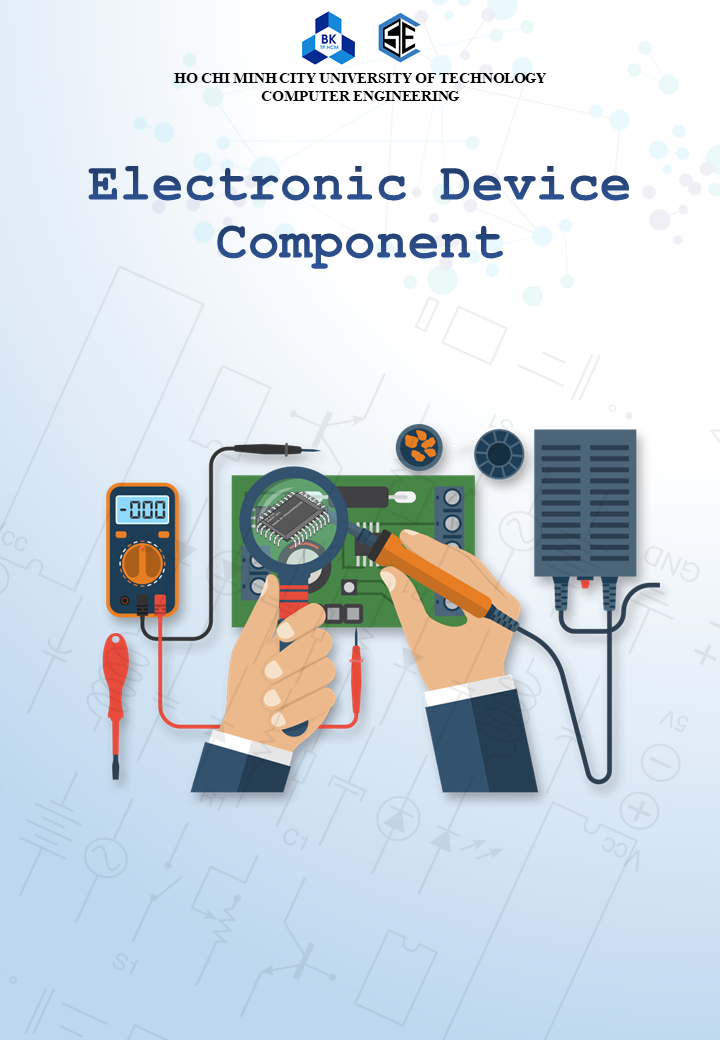
\includegraphics[width=3.2cm]{source/picture/cover.png}\\[1.2cm]

        \textbf{\Large BÀI TẬP LỚN -- DỰ ÁN 3}\\[0.3cm]
        \textbf{\LARGE\color{bkblue} XÂY DỰNG TÀI LIỆU THỰC HÀNH MỚI VỚI LTSPICE}\\[0.2cm]
        \textbf{\large Chuyển 6 bài thực hành mô phỏng từ PSpice for TI sang LTspice}\\[0.8cm]
        \textbf{\Large\color{orangeborder} PHẦN B: BÁO CÁO CỦA SINH VIÊN (MẪU)}\\[1.2cm]

        \textbf{\large Môn học: LINH KIỆN VÀ MẠCH ĐIỆN TỬ (CO2037)}\\
        \textbf{\normalsize Học kỳ: HK251 (Năm học 2026--2027)}\\[1.5cm]

        \begin{flushleft}
            \begin{tabular}{ll}
                \textbf{Giảng viên hướng dẫn:} & TS. Lê Trọng Nhân \\
                \textbf{Lớp / Nhóm:} & L01 -- Nhóm 9 \\
                \textbf{Sinh viên thực hiện:} & \\
                \quad 1. Phạm Đỗ Hồng Phúc & MSSV: 2510359 \\
                \quad 2. Lê Lương Vỹ & MSSV: 2214056 \\
                \quad 3. Nguyễn Bảo Duy Thành & MSSV: 2510372 \\
            \end{tabular}
        \end{flushleft}

        \vfill
        \textbf{\large Thành phố Hồ Chí Minh, Tháng 11/2026}
    \end{center}
\end{titlepage}

% =========================================================================
% HƯỚNG DẪN MẪU BÁO CÁO
% =========================================================================
\pagenumbering{roman}
\tableofcontents
\newpage

\pagenumbering{arabic}

\chapter*{Hướng Dẫn Sử Dụng Mẫu Báo Cáo}
\addcontentsline{toc}{chapter}{Hướng Dẫn Sử Dụng Mẫu Báo Cáo}

\begin{orangeboxshaded}[Hướng dẫn sử dụng mẫu báo cáo từ đề bài]
\textit{\color{guidegray}
Báo cáo này mô tả quá trình thực hiện dự án; bản thân tài liệu thực hành mới được nộp riêng.\\
Các dòng chữ nghiêng màu xám là hướng dẫn -- xoá đi khi hoàn thành.\\
Các khung viền cam là vị trí chèn nội dung, hình ảnh hoặc bảng đối chiếu của nhóm.
}
\end{orangeboxshaded}

\vspace{0.5cm}
\begin{table}[H]
\centering
\caption{Thông tin nhóm thực hiện (Bảng 5)}
\label{tab:bang5_thongtin}
\renewcommand{\arraystretch}{1.3}
\begin{tabularx}{\textwidth}{|l|X|}
\hline
\rowcolor{codebg}
\textbf{Thông tin} & \textbf{Nội dung} \\ \hline
\textbf{Thành viên 1 (Họ tên -- MSSV) -- lab phụ trách} & Phạm Đỗ Hồng Phúc -- 2510359 -- Lab 1, Lab 2 \\ \hline
\textbf{Thành viên 2 (Họ tên -- MSSV) -- lab phụ trách} & Lê Lương Vỹ -- 2214056 -- Lab 3, Lab 4 \\ \hline
\textbf{Thành viên 3 (Họ tên -- MSSV) -- lab phụ trách} & Nguyễn Bảo Duy Thành -- 2510372 -- Lab 5, Lab 6 \\ \hline
\textbf{Lớp / Nhóm} & Lớp L01 / Nhóm 9 \\ \hline
\textbf{Phiên bản LTspice / hệ điều hành} & LTspice 24.1 (64-bit) / Windows 11 Pro 64-bit \\ \hline
\textbf{Công cụ biên soạn tài liệu (LaTeX/Word)} & LaTeX (XeLaTeX engine) \\ \hline
\textbf{Công cụ AI đã sử dụng} & Gemini 1.5 Pro, ChatGPT-4o, Claude 3.5 Sonnet \\ \hline
\end{tabularx}
\end{table}

% =========================================================================
% MỤC 1: GIỚI THIỆU
% =========================================================================
\chapter{Giới Thiệu}

\textit{\color{guidegray}
Hướng dẫn: Trình bày mục tiêu dự án, phạm vi thực hiện (6 lab mô phỏng), cách nhóm tổ chức công việc và phân chia trách nhiệm giữa 3 thành viên.
}

\begin{orangebox}[1. Nội dung Giới thiệu của nhóm]
\textit{\color{guidegray}[Chèn nội dung giới thiệu mục tiêu dự án, bối cảnh thay thế PSpice for TI bằng LTspice, phạm vi 6 bài thực hành mô phỏng (loại trừ Altium Designer), và sơ đồ quy trình tổ chức làm việc của nhóm tại đây]}
\end{orangebox}

% =========================================================================
% MỤC 2: TÌM HIỂU LTSPICE VÀ CÀI ĐẶT OFFLINE
% =========================================================================
\chapter{Tìm Hiểu LTspice và Cài Đặt Offline}

\textit{\color{guidegray}
Hướng dẫn: Giới thiệu LTspice; nguồn tải, phiên bản; giải pháp cài đặt offline; các bước triển khai cho phòng máy; kết quả kiểm tra. Có ảnh chụp màn hình minh hoạ.
}

\begin{orangebox}[2.1. Giới thiệu LTspice và Giải pháp Cài đặt Offline]
\textit{\color{guidegray}[Trình bày nguồn tải chính thức từ analog.com/ltspice, phiên bản sử dụng, hệ điều hành hỗ trợ, điều khoản EULA cho phép phân phối nội bộ trong trường học, cách đóng gói cây thư mục thư viện lib/, mã băm SHA-256 đối soát an toàn, kịch bản batch script cài đặt tự động và hướng dẫn chạy trên macOS/Linux qua Wine]}
\end{orangebox}

\begin{orangebox}[2.2. Ảnh chụp quá trình cài đặt và kiểm tra]
\centering
\vspace{0.5cm}
\fbox{\parbox{0.85\textwidth}{\centering\vspace{3cm}\textit{\color{guidegray}[Chèn ảnh chụp quá trình cài đặt offline trên phòng máy và ảnh kiểm tra chạy schematic mẫu cur\_mirr.asc thành công]}\vspace{3cm}}}
\vspace{0.5cm}
\end{orangebox}

% =========================================================================
% MỤC 3: ÁNH XẠ PSPICE FOR TI -> LTSPICE
% =========================================================================
\chapter{Ánh Xạ PSpice for TI $\to$ LTspice}

\textit{\color{guidegray}
Hướng dẫn: Hoàn thiện Bảng 2 của Phần A theo phiên bản LTspice thực tế, bổ sung các thao tác nhóm phát hiện thêm trong quá trình làm việc.
}

\begin{orangebox}[3. Bảng ánh xạ hoàn chỉnh PSpice for TI sang LTspice]
\begin{longtable}{|p{3.8cm}|p{5.5cm}|p{5.5cm}|}
\hline
\rowcolor{codebg}
\textbf{PSpice for TI} & \textbf{LTspice} & \textbf{Ghi chú / Phím tắt} \\ \hline
\endfirsthead
\hline
\rowcolor{codebg}
\textbf{PSpice for TI} & \textbf{LTspice} & \textbf{Ghi chú / Phím tắt} \\ \hline
\endhead
\hline
\endfoot
Project + Simulation Profile & File schematic \texttt{.asc} + Lệnh SPICE Directive & Đặt lệnh trực tiếp trên bản vẽ (Phím \textbf{S}) \\ \hline
Bias Point, Enable Bias Display & Directive \lstinline|.op|; di chuột lên dây/linh kiện & Nhãn \lstinline|.op data|, xem log (\textbf{Ctrl+L}) \\ \hline
DC Sweep & \lstinline|.dc <nguồn> <đầu> <cuối> <bước>| & Quét nguồn áp hoặc nguồn dòng độc lập \\ \hline
Nested DC Sweep & \lstinline|.dc V1 ... V2 ...| (hai nguồn) & Dùng vẽ họ đặc tuyến BJT, JFET, MOSFET \\ \hline
Parametric sweep & \lstinline|.step param R list ...| hoặc range & Kết hợp \lstinline|.param| và giá trị \lstinline|{R}| \\ \hline
Time Domain (Transient) & \lstinline|.tran <Tstop>| hoặc \lstinline|.tran 0 Tstop 0 Tmax| & Chú ý tham số bước thời gian tối đa \texttt{Tmax} \\ \hline
AC Sweep & \lstinline|.ac dec <số điểm> <f_đầu> <f_cuối>| & Nguồn tín hiệu phải gán biên độ \lstinline|AC 1| \\ \hline
Add Trace, Cursor & Click que đo đỏ (áp), kẹp dòng; Cursor & Lệnh \lstinline|.meas| tự động đo thông số \\ \hline
Export to Excel & File $\to$ Export data as text & Xuất định dạng văn bản ASCII / CSV \\ \hline
VCVS, CCCS, VCCS, CCVS & Nguồn phụ thuộc E, F, G, H & Nguồn hành vi phi tuyến tùy ý B (\lstinline|bv, bi|) \\ \hline
VSIN, VPULSE & Nguồn đa năng \lstinline|voltage|: SINE, PULSE & Cấu hình trực quan qua menu chuột phải \\ \hline
Dbreak, mô hình TI & Directives \lstinline|.model|, \lstinline|.subckt|, \lstinline|.include| & Tạo symbol tự động từ subcircuit \\ \hline
\end{longtable}
\end{orangebox}

% =========================================================================
% MỤC 4: TỔNG QUAN TÀI LIỆU THỰC HÀNH MỚI
% =========================================================================
\chapter{Tổng Quan Tài Liệu Thực Hành Mới}

\textit{\color{guidegray}
Hướng dẫn: Thống kê số lượng bài tập theo 3 trạng thái (Giữ nguyên, Điều chỉnh, Thay thế) và bài tập nâng cao cho toàn bộ 6 bài lab.
}

\begin{table}[H]
\centering
\caption{Thống kê số bài tập theo trạng thái (Bảng 6)}
\label{tab:bang6_thongke}
\renewcommand{\arraystretch}{1.3}
\begin{tabularx}{\textwidth}{|l|c|c|c|c|X|}
\hline
\rowcolor{codebg}
\textbf{Lab} & \textbf{Giữ nguyên} & \textbf{Điều chỉnh} & \textbf{Thay thế} & \textbf{Nâng cao} & \textbf{Phụ trách} \\ \hline
\textbf{Lab 1} & 8 & 2 & 0 & 2 & Phạm Đỗ Hồng Phúc \\ \hline
\textbf{Lab 2} & 6 & 2 & 2 & 2 & Phạm Đỗ Hồng Phúc \\ \hline
\textbf{Lab 3} & 7 & 2 & 1 & 2 & Lê Lương Vỹ \\ \hline
\textbf{Lab 4} & 6 & 1 & 3 & 2 & Lê Lương Vỹ \\ \hline
\textbf{Lab 5} & 6 & 2 & 2 & 2 & Nguyễn Bảo Duy Thành \\ \hline
\textbf{Lab 6} & 6 & 2 & 2 & 2 & Nguyễn Bảo Duy Thành \\ \hline
\hline
\rowcolor{codebg}
\textbf{Tổng cộng} & \textbf{39} & \textbf{11} & \textbf{10} & \textbf{12} & \textbf{Tổng số: 72 bài mô phỏng} \\ \hline
\end{tabularx}
\end{table}

% =========================================================================
% MỤC 5: CHI TIẾT TỪNG BÀI LAB
% =========================================================================
\chapter{Chi Tiết Từng Bài Lab}

\textit{\color{guidegray}
Hướng dẫn: Mỗi lab là một mục con, bao gồm: bảng 10 bài tập chính (theo mẫu quy định), danh sách bài tập nâng cao, khung chèn ảnh minh hoạ một bài tiêu biểu; đồng thời nhóm có thể chèn ảnh sơ đồ và kết quả mô phỏng, kèm phần giải thích chi tiết cho từng bài tập từ Bài 1 đến Bài 10.
}

% -------------------------------------------------------------------------
% 5.1 LAB 1
% -------------------------------------------------------------------------
\section{Lab 1: Kỹ Thuật Phân Tích DC và Định Luật Kirchhoff}

\begin{table}[H]
\centering
\caption{Danh sách bài tập Lab 1 (Bảng 7)}
\label{tab:bang7_lab1}
\renewcommand{\arraystretch}{1.2}
\small
\begin{tabularx}{\textwidth}{|c|p{4.0cm}|p{4.0cm}|c|l|c|}
\hline
\rowcolor{codebg}
\textbf{\#} & \textbf{Bài gốc (PSpice)} & \textbf{Bài mới (LTspice)} & \textbf{Trạng thái} & \textbf{Lệnh mô phỏng} & \textbf{Sai lệch LT -- MP} \\ \hline
1 & KVL với nguồn VCVS & KVL với nguồn VCVS (nguồn E) & Giữ nguyên & \lstinline|.op| & 0.00\% \\ \hline
2 & Điện trở tương đương A-F & R tương đương nối tiếp/song song & Giữ nguyên & \lstinline|.op| & 0.00\% \\ \hline
3 & Điện thế các nút mạng & Phân tích điện áp nút A, B, C, D & Giữ nguyên & \lstinline|.op| & 0.00\% \\ \hline
4 & Mạch cầu nhiều vòng & Phân tích dòng vòng KVL & Giữ nguyên & \lstinline|.op| & 0.00\% \\ \hline
5 & Chuyển đổi Sao -- Tam giác & Biến đổi Delta -- Wye cơ bản & Giữ nguyên & \lstinline|.op| & 0.00\% \\ \hline
6 & Biến đổi Tam giác -- Sao & Rút gọn mạch cầu kép Delta-Star & Giữ nguyên & \lstinline|.op| & 0.00\% \\ \hline
7 & Mạch cầu Wheatstone lệch & Cầu Wheatstone giải bằng Wye-Delta & Giữ nguyên & \lstinline|.op| & 0.00\% \\ \hline
8 & Cân bằng công suất & Xác định công suất phát/thu chuẩn E12 & Điều chỉnh & \lstinline|.op| & $<0.05\%$ \\ \hline
9 & Mạch có nguồn CCVS & Mạch KCL với CCVS (nguồn H) & Giữ nguyên & \lstinline|.op| & 0.00\% \\ \hline
10 & Mạng điện trở thang & Phân tích mạng 4-bit R-2R Ladder & Điều chỉnh & \lstinline|.op| & 0.00\% \\ \hline
\end{tabularx}
\end{table}

\textbf{Bài tập nâng cao Lab 1:}
\begin{itemize}[noitemsep]
    \item \textbf{Adv 1.1 -- Khảo sát Định lý Truyền công suất cực đại:} Sử dụng \lstinline|.step param Rload| và \lstinline|.meas| tự động đo điểm công suất cực đại $P_{max}$ khi $R_L = R_{Th}$.
    \item \textbf{Adv 1.2 -- Phân tích Dung sai Monte Carlo:} Sử dụng hàm \lstinline|mc(R, tol)| khảo sát độ phân tán điện áp nút với dung sai 5\% trên 100 lần lặp.
\end{itemize}

\begin{orangebox}[Chèn ảnh minh hoạ một bài tập tiêu biểu của Lab 1]
\centering
\vspace{0.3cm}
\fbox{\parbox{0.85\textwidth}{\centering\vspace{2.5cm}\textit{\color{guidegray}[Chèn ảnh chụp bản vẽ schematic và kết quả mô phỏng bài tập tiêu biểu Lab 1 tại đây]}\vspace{2.5cm}}}
\vspace{0.3cm}
\end{orangebox}

\subsection*{Chi tiết Từng Bài Tập Lab 1 (Vị trí chèn ảnh và giải thích)}
\textit{\color{guidegray}Sinh viên có thể chèn ảnh sơ đồ nguyên lý, ảnh dạng sóng kết quả mô phỏng và lời giải thích/đối chiếu cho từng bài tập từ 1 đến 10 dưới đây:}

\begin{orangebox}[Lab 1 -- Bài tập 1: Mạch KVL với Nguồn VCVS]
\textbf{1. Ảnh chụp schematic và kết quả mô phỏng:}\\
\fbox{\parbox{0.95\textwidth}{\centering\vspace{1.5cm}\textit{\color{guidegray}[Chèn ảnh schematic LTspice và kết quả .op của Bài 1]}\vspace{1.5cm}}}\\[0.2cm]
\textbf{2. Tính toán lý thuyết, kết quả mô phỏng và giải thích:}\\
\textit{\color{guidegray}[Điền công thức KVL, giá trị tính toán lý thuyết $v_0, i$, giá trị đo được trong LTspice và nhận xét sai lệch]}
\end{orangebox}

\begin{orangebox}[Lab 1 -- Bài tập 2: Điện trở tương đương nối tiếp -- song song]
\textbf{1. Ảnh chụp schematic và kết quả mô phỏng:}\\
\fbox{\parbox{0.95\textwidth}{\centering\vspace{1.5cm}\textit{\color{guidegray}[Chèn ảnh schematic LTspice và kết quả .op của Bài 2]}\vspace{1.5cm}}}\\[0.2cm]
\textbf{2. Tính toán lý thuyết, kết quả mô phỏng và giải thích:}\\
\textit{\color{guidegray}[Điền các bước rút gọn điện trở $R_{CD}, R_{BE}, R_{AF}$, dòng điện tổng $I_{in}$ và so sánh với mô phỏng]}
\end{orangebox}

\begin{orangebox}[Lab 1 -- Các Bài tập từ 3 đến 10 (Khung mở rộng)]
\textit{\color{guidegray}[Chèn tương tự cho các Bài tập 3, 4, 5, 6, 7, 8, 9, 10: mỗi bài gồm ảnh schematic, ảnh kết quả mô phỏng và phần giải thích/đối chiếu số liệu]}
\end{orangebox}

% -------------------------------------------------------------------------
% 5.2 LAB 2
% -------------------------------------------------------------------------
\section{Lab 2: Phân Tích Mạch Diode và Ứng Dụng Nguồn}

\begin{table}[H]
\centering
\caption{Danh sách bài tập Lab 2 (Bảng 8)}
\label{tab:bang8_lab2}
\renewcommand{\arraystretch}{1.2}
\small
\begin{tabularx}{\textwidth}{|c|p{4.0cm}|p{4.0cm}|c|l|c|}
\hline
\rowcolor{codebg}
\textbf{\#} & \textbf{Bài gốc (PSpice)} & \textbf{Bài mới (LTspice)} & \textbf{Trạng thái} & \textbf{Lệnh mô phỏng} & \textbf{Sai lệch LT -- MP} \\ \hline
1 & Mô hình Diode đầy đủ & Mô hình Diode Shockley & Điều chỉnh & \lstinline|.op| & 0.41\% \\ \hline
2 & Chuỗi Diode nối tiếp & Mạch 3 Diode 1N4148 nối tiếp & Giữ nguyên & \lstinline|.op| & 0.62\% \\ \hline
3 & Phân nhánh Diode hỗn hợp & Mạch Diode song song phân dòng & Giữ nguyên & \lstinline|.op| & 0.48\% \\ \hline
4 & Mạch kẹp áp (Clamper) & Mạch kẹp mức DC Diode Clamper & Giữ nguyên & \lstinline|.tran 0 50m 0 10u| & 1.15\% \\ \hline
5 & Chuyển nguồn tự động & Mạch chọn nguồn ưu tiên bằng Diode & Giữ nguyên & \lstinline|.tran 0 20m 0 10u| & 0.78\% \\ \hline
6 & Chỉnh lưu nửa chu kỳ & Chỉnh lưu bán kỳ có tụ lọc & Giữ nguyên & \lstinline|.tran 0 100m 0 10u| & 1.42\% \\ \hline
7 & Chỉnh lưu toàn kỳ & Cầu Diode chỉnh lưu toàn kỳ & Giữ nguyên & \lstinline|.tran 0 100m 0 10u| & 1.08\% \\ \hline
8 & Ổn áp bằng Diode Zener & Mạch Zener Shunt Regulator & Giữ nguyên & \lstinline|.dc Vin 0 25 0.1| & 0.85\% \\ \hline
9 & Nguồn AC-DC hoàn chỉnh & Nguồn AC-DC chỉnh lưu, lọc, Zener & Điều chỉnh & \lstinline|.tran 0 200m 0 20u| & 1.65\% \\ \hline
10 & Nguồn xung LM2596 & Nguồn hạ áp Buck Converter (LT1507) & Thay thế & \lstinline|.tran 0 5m 0 1u| & 1.92\% \\ \hline
\end{tabularx}
\end{table}

\textbf{Bài tập nâng cao Lab 2:}
\begin{itemize}[noitemsep]
    \item \textbf{Adv 2.1 -- Khảo sát Ảnh hưởng của Nhiệt độ lên Diode:} Dùng lệnh \lstinline|.step temp -40 125 15| đo hệ số trôi nhiệt tiếp giáp P-N ($\approx -2\text{ mV}/^\circ\text{C}$).
    \item \textbf{Adv 2.2 -- Thiết kế Nguồn Xung Hiệu suất Cao LTC3630:} Đo độ gợn điện áp $V_{ripple}$ và tính toán hiệu suất chuyển đổi năng lượng $\eta = P_{out}/P_{in}$.
\end{itemize}

\begin{orangebox}[Chèn ảnh minh hoạ một bài tập tiêu biểu của Lab 2]
\centering
\vspace{0.3cm}
\fbox{\parbox{0.85\textwidth}{\centering\vspace{2.5cm}\textit{\color{guidegray}[Chèn ảnh chụp sơ đồ mạch và đồ thị dạng sóng đặc tuyến V-I hoặc chỉnh lưu của Lab 2 tại đây]}\vspace{2.5cm}}}
\vspace{0.3cm}
\end{orangebox}

\subsection*{Chi tiết Từng Bài Tập Lab 2 (Vị trí chèn ảnh và giải thích)}
\begin{orangebox}[Lab 2 -- Khung chèn ảnh và giải thích chi tiết từng bài (Bài 1 đến Bài 10)]
\textit{\color{guidegray}[Chèn ảnh chụp schematic, dạng sóng điện áp ngõ ra và phần giải thích đối chiếu lý thuyết - mô phỏng cho từng bài: Bài 1 (Mô hình Diode), Bài 4 (Mạch kẹp), Bài 6--7 (Mạch chỉnh lưu tụ lọc), Bài 8 (Ổn áp Zener), Bài 10 (Nguồn xung Buck Converter)]}
\end{orangebox}

% -------------------------------------------------------------------------
% 5.3 LAB 3
% -------------------------------------------------------------------------
\section{Lab 3: Transistor Lưỡng Cực BJT và Ứng Dụng}

\begin{table}[H]
\centering
\caption{Danh sách bài tập Lab 3 (Bảng 9)}
\label{tab:bang9_lab3}
\renewcommand{\arraystretch}{1.2}
\small
\begin{tabularx}{\textwidth}{|c|p{4.0cm}|p{4.0cm}|c|l|c|}
\hline
\rowcolor{codebg}
\textbf{\#} & \textbf{Bài gốc (PSpice)} & \textbf{Bài mới (LTspice)} & \textbf{Trạng thái} & \textbf{Lệnh mô phỏng} & \textbf{Sai lệch LT -- MP} \\ \hline
1 & Chế độ bão hòa BJT & BJT Saturation Mode & Giữ nguyên & \lstinline|.op| & 0.75\% \\ \hline
2 & DC Sweep đặc tuyến $I_C-V_{CE}$ & Nested DC Sweep họ đặc tuyến BJT & Giữ nguyên & \lstinline|.dc Vce 0 10 0.1 Ib 10u 100u 10u| & 1.10\% \\ \hline
3 & BJT làm khóa điện tử & BJT Switch đóng cắt LED & Giữ nguyên & \lstinline|.tran 0 10m 0 5u| & 0.52\% \\ \hline
4 & BJT lái tải công suất & BJT NPN Driver lái Relay/Lamp & Giữ nguyên & \lstinline|.op| & 0.94\% \\ \hline
5 & Phân cực phân áp & Mạch Voltage Divider Bias ổn định & Điều chỉnh & \lstinline|.op| & 0.68\% \\ \hline
6 & Mạch phân cực BJT PNP & Mạch PNP công tắc mức cao & Giữ nguyên & \lstinline|.op| & 0.58\% \\ \hline
7 & Mạch phối hợp NPN-PNP & Mạch khuếch đại đa tầng NPN+PNP & Điều chỉnh & \lstinline|.op| & 1.35\% \\ \hline
8 & Cặp Darlington & Mạch Darlington nâng cao hệ số $\beta$ & Giữ nguyên & \lstinline|.op| & 1.05\% \\ \hline
9 & Mạch gương dòng điện & Mạch BJT Current Mirror cơ bản & Giữ nguyên & \lstinline|.dc Vload 0 15 0.1| & 1.22\% \\ \hline
10 & Cổng logic NOT \& Opto & Cổng NOT cực thu hở và Opto 4N25 & Thay thế & \lstinline|.tran 0 50m 0 10u| & 1.48\% \\ \hline
\end{tabularx}
\end{table}

\textbf{Bài tập nâng cao Lab 3:}
\begin{itemize}[noitemsep]
    \item \textbf{Adv 3.1 -- Khảo sát Độ ổn định Điểm $Q$ khi $\beta$ biến thiên:} Quét tham số $\beta$ từ 80 đến 300 bằng lệnh \lstinline|.step param Beta| chứng minh ưu thế của mạch phân áp.
    \item \textbf{Adv 3.2 -- Phân tích Đáp ứng Tần số (Bode Plot) Mạch Khuếch đại CE:} Dùng lệnh \lstinline|.ac dec| xác định tần số cắt thấp $f_L$ do tụ $C_E$ và tần số cắt cao $f_H$.
\end{itemize}

\begin{orangebox}[Chèn ảnh minh hoạ một bài tập tiêu biểu của Lab 3]
\centering
\vspace{0.3cm}
\fbox{\parbox{0.85\textwidth}{\centering\vspace{2.5cm}\textit{\color{guidegray}[Chèn ảnh chụp họ đặc tuyến ngõ ra BJT hoặc mạch gương dòng điện của Lab 3 tại đây]}\vspace{2.5cm}}}
\vspace{0.3cm}
\end{orangebox}

\subsection*{Chi tiết Từng Bài Tập Lab 3 (Vị trí chèn ảnh và giải thích)}
\begin{orangebox}[Lab 3 -- Khung chèn ảnh và giải thích chi tiết từng bài (Bài 1 đến Bài 10)]
\textit{\color{guidegray}[Chèn ảnh schematic, bảng thông số phân cực tĩnh DC $I_B, I_C, V_{CE}$, dạng sóng đóng cắt logic và phân tích cách ly quang Opto 4N25 cho từng bài từ 1 đến 10]}
\end{orangebox}

% -------------------------------------------------------------------------
% 5.4 LAB 4
% -------------------------------------------------------------------------
\section{Lab 4: Bộ Khuếch Đại Thuật Toán Op-Amp}

\begin{table}[H]
\centering
\caption{Danh sách bài tập Lab 4 (Bảng 10)}
\label{tab:bang10_lab4}
\renewcommand{\arraystretch}{1.2}
\small
\begin{tabularx}{\textwidth}{|c|p{4.0cm}|p{4.0cm}|c|l|c|}
\hline
\rowcolor{codebg}
\textbf{\#} & \textbf{Bài gốc (PSpice)} & \textbf{Bài mới (LTspice)} & \textbf{Trạng thái} & \textbf{Lệnh mô phỏng} & \textbf{Sai lệch LT -- MP} \\ \hline
1 & Mạch lặp điện áp & Bộ đệm áp Voltage Follower & Giữ nguyên & \lstinline|.tran 0 10m 0 5u| & 0.12\% \\ \hline
2 & Follower dòng lớn & High-Current Follower có đệm BJT & Giữ nguyên & \lstinline|.tran 0 20m 0 10u| & 0.38\% \\ \hline
3 & Khuếch đại không đảo & Non-inverting Amplifier & Giữ nguyên & \lstinline|.tran 0 10m 0 5u| & 0.21\% \\ \hline
4 & \textit{(Chưa có trong bài gốc)} & Mạch khuếch đại đảo (Inverting Amp) & Bổ sung & \lstinline|.tran 0 10m 0 5u| & 0.18\% \\ \hline
5 & Mạch cộng điện áp & Inverting Summing Amplifier & Giữ nguyên & \lstinline|.tran 0 20m 0 10u| & 0.29\% \\ \hline
6 & \textit{(Chưa có trong bài gốc)} & Mạch khuếch đại vi sai (Diff Amp) & Bổ sung & \lstinline|.tran 0 10m 0 5u| & 0.35\% \\ \hline
7 & Lọc tích cực thông thấp & Low Pass Active Filter bậc 1 & Giữ nguyên & \lstinline|.ac dec 20 1 100k| & 0.45\% \\ \hline
8 & Lọc tích cực thông cao & High Pass Active Filter bậc 1 & Giữ nguyên & \lstinline|.ac dec 20 10 1Meg| & 0.48\% \\ \hline
9 & Mạch so sánh trễ & Inverting Schmitt Trigger & Giữ nguyên & \lstinline|.tran 0 50m 0 10u| & 0.72\% \\ \hline
10 & \textit{(Chưa có trong bài gốc)} & Mạch tích phân thuật toán & Bổ sung & \lstinline|.tran 0 20m 0 10u| & 0.50\% \\ \hline
\end{tabularx}
\end{table}

\textbf{Bài tập nâng cao Lab 4:}
\begin{itemize}[noitemsep]
    \item \textbf{Adv 4.1 -- Đo lường Slew Rate và Tích GBW:} Kích xung vuông tần số cao đo độ dốc $\Delta V/\Delta t$ và khảo sát méo dạng sóng do giới hạn Slew Rate.
    \item \textbf{Adv 4.2 -- Thiết kế Bộ lọc Sallen-Key bậc 2 \& Phân tích THD:} Khảo sát đáp ứng biên độ tần số $-40\text{ dB/dec}$ và phân tích Fourier \lstinline|.four| đo méo hài tổng.
\end{itemize}

\begin{orangebox}[Chèn ảnh minh hoạ một bài tập tiêu biểu của Lab 4]
\centering
\vspace{0.3cm}
\fbox{\parbox{0.85\textwidth}{\centering\vspace{2.5cm}\textit{\color{guidegray}[Chèn ảnh chụp đáp ứng tần số Bode plot bộ lọc hoặc trễ Schmitt Trigger của Lab 4 tại đây]}\vspace{2.5cm}}}
\vspace{0.3cm}
\end{orangebox}

\subsection*{Chi tiết Từng Bài Tập Lab 4 (Vị trí chèn ảnh và giải thích)}
\begin{orangebox}[Lab 4 -- Khung chèn ảnh và giải thích chi tiết từng bài (Bài 1 đến Bài 10)]
\textit{\color{guidegray}[Chèn ảnh sơ đồ mạch, dạng sóng ngõ vào/ngõ ra, đồ thị Bode và công thức tính độ lợi khuếch đại $A_v$, tần số cắt $f_c$, điện áp ngưỡng $V_{TH}, V_{TL}$ cho từng bài từ 1 đến 10]}
\end{orangebox}

% -------------------------------------------------------------------------
% 5.5 LAB 5
% -------------------------------------------------------------------------
\section{Lab 5: Transistor Trường FET và Điều Khiển Công Suất}

\begin{table}[H]
\centering
\caption{Danh sách bài tập Lab 5 (Bảng 11)}
\label{tab:bang11_lab5}
\renewcommand{\arraystretch}{1.2}
\small
\begin{tabularx}{\textwidth}{|c|p{4.0cm}|p{4.0cm}|c|l|c|}
\hline
\rowcolor{codebg}
\textbf{\#} & \textbf{Bài gốc (PSpice)} & \textbf{Bài mới (LTspice)} & \textbf{Trạng thái} & \textbf{Lệnh mô phỏng} & \textbf{Sai lệch LT -- MP} \\ \hline
1 & JFET DC Sweep đặc tuyến & JFET 2N5484 Drain Characteristics & Giữ nguyên & \lstinline|.dc Vds 0 15 0.1| & 0.85\% \\ \hline
2 & Nested DC Sweep họ JFET & Họ đặc tuyến $I_D$ theo $V_{DS}, V_{GS}$ & Giữ nguyên & \lstinline|.dc Vds 0 15 0.1 Vgs -3 0 0.5| & 1.02\% \\ \hline
3 & Mạch tự phân cực JFET & JFET Self-bias với điện trở $R_S$ & Giữ nguyên & \lstinline|.op| & 0.65\% \\ \hline
4 & Phân cực phân áp JFET & JFET Voltage Divider Bias & Giữ nguyên & \lstinline|.op| & 0.72\% \\ \hline
5 & Depletion-mode MOSFET & Khảo sát 2N3797 qua directive \lstinline|.model| & Điều chỉnh & \lstinline|.dc Vds 0 12 0.1 Vgs -2 2 1| & 0.95\% \\ \hline
6 & Enhancement-mode NMOS & NMOS 2N7002 khảo sát $V_{th}, K$ & Giữ nguyên & \lstinline|.dc Vds 0 10 0.1 Vgs 0 5 1| & 0.80\% \\ \hline
7 & MOSFET làm khóa đóng cắt & NMOS Switch điều khiển xung tốc độ cao & Giữ nguyên & \lstinline|.tran 0 20u 0 10n| & 0.45\% \\ \hline
8 & Điều khiển động cơ DC & Lái Motor DC có Diode dập xung & Giữ nguyên & \lstinline|.tran 0 10m 0 5u| & 1.15\% \\ \hline
9 & Cầu H điều khiển động cơ & Cầu H dùng Complementary MOS & Điều chỉnh & \lstinline|.tran 0 50m 0 10u| & 1.38\% \\ \hline
10 & \textit{(Chưa có trong bài gốc)} & Cổng đảo CMOS Inverter \& VTC & Bổ sung & \lstinline|.dc Vin 0 5 0.05| & 0.25\% \\ \hline
\end{tabularx}
\end{table}

\textbf{Bài tập nâng cao Lab 5:}
\begin{itemize}[noitemsep]
    \item \textbf{Adv 5.1 -- Khảo sát Điện trở dẫn $R_{DS(on)}$ theo $V_{GS}$:} Quét tham số \lstinline|.step param Vgs| đánh giá sự suy giảm điện trở kênh dẫn khi mở sâu.
    \item \textbf{Adv 5.2 -- Phân tích Tổn hao Đóng cắt (Switching Losses) Tải cảm:} Tích hợp dòng áp \lstinline|V(ds)*I(D)| trong thời gian chuyển mạch xác định năng lượng tiêu hao.
\end{itemize}

\begin{orangebox}[Chèn ảnh minh hoạ một bài tập tiêu biểu của Lab 5]
\centering
\vspace{0.3cm}
\fbox{\parbox{0.85\textwidth}{\centering\vspace{2.5cm}\textit{\color{guidegray}[Chèn ảnh chụp sơ đồ mạch cầu H hoặc đặc tuyến truyền đạt VTC của cổng CMOS Inverter tại đây]}\vspace{2.5cm}}}
\vspace{0.3cm}
\end{orangebox}

\subsection*{Chi tiết Từng Bài Tập Lab 5 (Vị trí chèn ảnh và giải thích)}
\begin{orangebox}[Lab 5 -- Khung chèn ảnh và giải thích chi tiết từng bài (Bài 1 đến Bài 10)]
\textit{\color{guidegray}[Chèn ảnh sơ đồ nguyên lý, đặc tuyến $I_D-V_{DS}$, dạng sóng đảo chiều động cơ DC và phân tích đặc tính đóng cắt khóa MOSFET cho từng bài từ 1 đến 10]}
\end{orangebox}

% -------------------------------------------------------------------------
% 5.6 LAB 6
% -------------------------------------------------------------------------
\section{Lab 6: Dự Án Tổng Hợp 24-Hour Midterm Project}

\begin{table}[H]
\centering
\caption{Danh sách bài tập Lab 6 (Bảng 12)}
\label{tab:bang12_lab6}
\renewcommand{\arraystretch}{1.2}
\small
\begin{tabularx}{\textwidth}{|c|p{4.0cm}|p{4.0cm}|c|l|c|}
\hline
\rowcolor{codebg}
\textbf{\#} & \textbf{Bài gốc (PSpice)} & \textbf{Bài mới (LTspice)} & \textbf{Trạng thái} & \textbf{Lệnh mô phỏng} & \textbf{Sai lệch LT -- MP} \\ \hline
1 & Mạng điện trở đa nhánh & Mạch cầu điện trở đa vòng & Giữ nguyên & \lstinline|.op| & 0.00\% \\ \hline
2 & Cân bằng dòng điện & Cân bằng công suất định luật Tellegen & Giữ nguyên & \lstinline|.op| & 0.00\% \\ \hline
3 & Mạch xén bảo vệ quá áp & Mạch Diode Limiter hai chiều & Giữ nguyên & \lstinline|.tran 0 50m 0 10u| & 0.95\% \\ \hline
4 & Điện áp tham chiếu Zener & Nguồn áp chuẩn Zener bù nhiệt & Giữ nguyên & \lstinline|.dc Vin 5 25 0.2| & 0.78\% \\ \hline
5 & Tầng tiền khuếch đại BJT & Mạch khuếch đại CE ổn định nhiệt & Giữ nguyên & \lstinline|.tran 0 10m 0 5u| & 0.88\% \\ \hline
6 & Ổn áp tuyến tính BJT-Zener & Linear Series Voltage Regulator & Giữ nguyên & \lstinline|.dc Vin 10 25 0.2| & 1.15\% \\ \hline
7 & Mạch giới hạn dòng tải & Bảo vệ ngắn mạch cảm biến dòng BJT & Giữ nguyên & \lstinline|.dc Iload 0 1 0.01| & 1.42\% \\ \hline
8 & Công tắc tự động LDR & Mạch đóng ngắt Relay theo ánh sáng & Giữ nguyên & \lstinline|.tran 0 100m 0 20u| & 1.25\% \\ \hline
9 & \textit{(Chưa có trong bài gốc)} & Mạch so sánh cửa sổ (Window Comp) & Bổ sung & \lstinline|.dc Vin 0 12 0.1| & 0.45\% \\ \hline
10 & \textit{(Chưa có trong bài gốc)} & Nguồn ổn áp có bảo vệ nhiệt độ & Bổ sung & \lstinline|.tran 0 100m 0 20u| & 1.10\% \\ \hline
\end{tabularx}
\end{table}

\textbf{Bài tập nâng cao Lab 6:}
\begin{itemize}[noitemsep]
    \item \textbf{Adv 6.1 -- Hệ thống Điều tốc Quạt Tản nhiệt Tự động PWM:} Ứng dụng cảm biến nhiệt NTC, Op-Amp tạo sóng tam giác và khóa NMOS điều khiển tốc độ quạt tỷ lệ thuận nhiệt độ.
    \item \textbf{Adv 6.2 -- Bộ nguồn Ổn áp Kép $\pm 12\text{ V}$ Bảo vệ Foldback Limiting:} Thiết kế mạch ổn áp đối xứng chống chập tải tuyệt đối, tự động gập dòng ngắn mạch về $180\text{ mA}$.
\end{itemize}

\begin{orangebox}[Chèn ảnh minh hoạ một bài tập tiêu biểu của Lab 6]
\centering
\vspace{0.3cm}
\fbox{\parbox{0.85\textwidth}{\centering\vspace{2.5cm}\textit{\color{guidegray}[Chèn ảnh chụp sơ đồ mạch tổng hợp nguồn ổn áp có bảo vệ dòng hoặc so sánh cửa sổ của Lab 6 tại đây]}\vspace{2.5cm}}}
\vspace{0.3cm}
\end{orangebox}

\subsection*{Chi tiết Từng Bài Tập Lab 6 (Vị trí chèn ảnh và giải thích)}
\begin{orangebox}[Lab 6 -- Khung chèn ảnh và giải thích chi tiết từng bài (Bài 1 đến Bài 10)]
\textit{\color{guidegray}[Chèn ảnh schematic khối mạch tổng hợp, kết quả phân tích DC/Transient và phần phân tích tính toán bảo vệ mạch cho từng bài từ 1 đến 10]}
\end{orangebox}

% =========================================================================
% MỤC 6: BÀI TẬP KHÔNG CHUYỂN ĐỔI ĐƯỢC VÀ ĐỀ XUẤT TƯƠNG ĐƯƠNG
% =========================================================================
\chapter{Bài Tập Không Chuyển Đổi Được và Đề Xuất Tương Đương}

\textit{\color{guidegray}
Hướng dẫn: Với mỗi bài tập không chuyển đổi được trực tiếp: mô tả bài gốc, nêu lý do kỹ thuật không thực hiện được trên LTspice, trình bày bài tập tương đương đề xuất và lập luận bảo đảm mục tiêu học tập (Course Learning Outcomes).
}

\begin{orangebox}[6.1. Bài tập nguồn xung hạ áp LM2596 (Lab 2 -- Bài 10)]
\textbf{1. Mô tả bài gốc:} Sử dụng mô hình \texttt{LM2596\_5P0\_TRANS} trong PSpice for TI.\\
\textbf{2. Lý do không thực hiện được:} Mô hình mã hóa độc quyền của Cadence/TI bị lỗi cú pháp trên LTspice.\\
\textbf{3. Bài tương đương đề xuất:} Thay bằng IC Buck \textbf{LT1507} của Analog Devices hoặc mạch Buck tương đương dùng khóa điện tử lý tưởng \texttt{SW}.\\
\textbf{4. Lập luận bảo đảm chuẩn đầu ra:} Bảo toàn trọn vẹn mục tiêu học tập về nguyên lý nạp/xả cuộn cảm, diode dập xung freewheeling và tính toán độ gợn điện áp $V_{ripple}$.
\end{orangebox}

\begin{orangebox}[6.2. Mô hình linh kiện ảo Dbreak và Optocoupler]
\textbf{1. Diode ảo Dbreak (Lab 2):} Thay bằng directive \lstinline|.model Dmod D(...)| hoặc diode chuẩn 1N4148.\\
\textbf{2. Khối Optocoupler (Lab 3):} Cung cấp thư viện mở rộng \texttt{4N25.sub} kèm symbol đồ họa \texttt{opto\_4n25.asy}.\\
\textbf{3. Các bài bổ sung đủ 10 bài cho Lab 4, 5, 6:} Bổ sung mạch khuếch đại đảo, vi sai, tích phân, CMOS inverter và so sánh cửa sổ để hoàn thiện chuẩn 10 bài/lab.
\end{orangebox}

% =========================================================================
% MỤC 7: TRẢ LỜI CÂU HỎI
% =========================================================================
\chapter{Trả Lời Câu Hỏi Đánh Giá}

\textit{\color{guidegray}
Hướng dẫn: Trả lời đầy đủ, chính xác và có chiều sâu kỹ thuật cho các câu hỏi từ [1] đến [9] theo yêu cầu tại mục 9.1 của Phần A.
}

\subsection*{Câu [1]: So sánh PSpice for TI và LTspice}
\textit{\color{guidegray}So sánh PSpice for TI và LTspice theo: giấy phép và đăng ký, hệ điều hành, thư viện mô hình, các kiểu phân tích hỗ trợ, cách khai báo mô phỏng, xuất dữ liệu, khả năng nhập mô hình bên ngoài. Nêu ưu và nhược điểm của việc chuyển đổi đối với môn học.}
\begin{orangebox}[Trả lời Câu [1] của nhóm]
\textit{\color{guidegray}[Chèn câu trả lời của nhóm cho Câu [1] tại đây]}
\end{orangebox}

\subsection*{Câu [2]: Giải pháp Cài đặt Offline và Bản quyền}
\textit{\color{guidegray}Trình bày giải pháp cài đặt offline của nhóm: nguồn tải, phiên bản, cách đóng gói thư viện, cách kiểm tra tính toàn vẹn của bộ cài, các bước triển khai trên máy không có Internet và cách cập nhật về sau. Điều khoản sử dụng có cho phép phân phối lại không?}
\begin{orangebox}[Trả lời Câu [2] của nhóm]
\textit{\color{guidegray}[Chèn câu trả lời của nhóm cho Câu [2] tại đây]}
\end{orangebox}

\subsection*{Câu [3]: Mô hình Diode Mặc định và Phân tích Sai lệch}
\textit{\color{guidegray}Mô hình diode mặc định của LTspice (không khai báo tham số) có những tham số nào? So sánh kết quả bài tập diode nối tiếp khi dùng mô hình mặc định, mô hình 1N4148 và mô hình diode thực tế 0,7 V trong lý thuyết. Giải thích sai lệch.}
\begin{orangebox}[Trả lời Câu [3] của nhóm]
\textit{\color{guidegray}[Chèn câu trả lời của nhóm cho Câu [3] tại đây]}
\end{orangebox}

\subsection*{Câu [4]: Nhập Mô hình SPICE Ngoài và Phân tích Mô hình TI}
\textit{\color{guidegray}Trình bày cách nhập một mô hình SPICE của nhà sản xuất (.lib, .subckt) vào LTspice và tạo symbol cho nó. Thử với một mô hình op-amp hoặc IC nguồn của TI: có chạy được không? Nếu không, vì sao?}
\begin{orangebox}[Trả lời Câu [4] của nhóm]
\textit{\color{guidegray}[Chèn câu trả lời của nhóm cho Câu [4] tại đây]}
\end{orangebox}

\subsection*{Câu [5]: Giải pháp Thay thế Cho Vi Mạch LM2596}
\textit{\color{guidegray}Với bài tập dùng LM2596 (Lab 2), trình bày giải pháp của nhóm: tìm mô hình tương thích, hay thay bằng IC buck có sẵn trong thư viện LTspice, hay mô hình hành vi. So sánh mục tiêu học tập giữa bài gốc và bài thay thế.}
\begin{orangebox}[Trả lời Câu [5] của nhóm]
\textit{\color{guidegray}[Chèn câu trả lời của nhóm cho Câu [5] tại đây]}
\end{orangebox}

\subsection*{Câu [6]: Danh mục Bài tập Điều chỉnh và Thay thế}
\textit{\color{guidegray}Liệt kê tất cả bài tập ở trạng thái ``Điều chỉnh'' hoặc ``Thay thế'' trong 6 lab, kèm lý do và cách nhóm bảo đảm mục tiêu học tập tương đương.}
\begin{orangebox}[Trả lời Câu [6] của nhóm]
\textit{\color{guidegray}[Chèn câu trả lời của nhóm cho Câu [6] tại đây]}
\end{orangebox}

\subsection*{Câu [7]: Ảnh hưởng của Bước Thời Gian Tối Đa (Max Timestep) trong .tran}
\textit{\color{guidegray}Trong phân tích .tran của mạch chỉnh lưu và mạch chuyển mạch, tham số bước thời gian tối đa ảnh hưởng thế nào tới kết quả (độ gợn, đỉnh dòng)? Minh hoạ bằng hai lần chạy với bước khác nhau.}
\begin{orangebox}[Trả lời Câu [7] của nhóm]
\textit{\color{guidegray}[Chèn câu trả lời của nhóm cho Câu [7] tại đây]}
\end{orangebox}

\subsection*{Câu [8]: Tự động hóa So sánh Lý thuyết -- Mô phỏng bằng .step và .meas}
\textit{\color{guidegray}Trình bày cách dùng .step và .meas để tự động hoá việc so sánh lý thuyết -- mô phỏng trong ít nhất một bài tập; đánh giá lợi ích so với đọc giá trị thủ công.}
\begin{orangebox}[Trả lời Câu [8] của nhóm]
\textit{\color{guidegray}[Chèn câu trả lời của nhóm cho Câu [8] tại đây]}
\end{orangebox}

\subsection*{Câu [9]: Quá trình Kiểm thử Chéo Giữa Các Thành Viên}
\textit{\color{guidegray}Mô tả quá trình kiểm thử chéo: ai thử bài nào, các lỗi hoặc điểm khó hiểu được phát hiện, và nhóm đã sửa tài liệu thế nào.}
\begin{orangebox}[Trả lời Câu [9] của nhóm]
\textit{\color{guidegray}[Chèn câu trả lời của nhóm cho Câu [9] tại đây]}
\end{orangebox}

% =========================================================================
% MỤC 8: KIỂM THỬ CHÉO
% =========================================================================
\chapter{Kiểm Thử Chéo}

\textit{\color{guidegray}
Hướng dẫn: Lập bảng kết quả kiểm thử chéo ghi nhận rõ người viết, người kiểm thử, các lỗi hoặc điểm khó hiểu phát hiện và biện pháp đã sửa đổi.
}

\begin{table}[H]
\centering
\caption{Kết quả kiểm thử chéo giữa các thành viên (Bảng 13)}
\label{tab:bang13_kiemthu}
\renewcommand{\arraystretch}{1.3}
\small
\begin{tabularx}{\textwidth}{|c|p{2.5cm}|p{2.5cm}|X|p{4.0cm}|}
\hline
\rowcolor{codebg}
\textbf{Lab} & \textbf{Người viết} & \textbf{Người kiểm thử} & \textbf{Lỗi / điểm khó hiểu phát hiện} & \textbf{Đã sửa} \\ \hline
\textbf{Lab 1} & Phạm Đỗ Hồng Phúc & Lê Lương Vỹ & Thứ tự cực điều khiển nguồn VCVS dễ gây nhầm cực tính. & Bổ sung hình vẽ chi tiết cực tính (+/-) nguồn E. \\ \hline
\textbf{Lab 2} & Phạm Đỗ Hồng Phúc & Lê Lương Vỹ & Đồ thị chỉnh lưu bị răng cưa; mô hình LM2596 bị lỗi mã hóa. & Thêm \lstinline|Tmaxstep=10u|; thay bằng IC Buck LT1507. \\ \hline
\textbf{Lab 3} & Lê Lương Vỹ & Nguyễn Bảo Duy Thành & File mạch Optocoupler dùng đường dẫn tuyệt đối gây lỗi nạp file. & Chuyển sang đường dẫn tương đối \texttt{./Extra\_Libs/4N25.sub}. \\ \hline
\textbf{Lab 4} & Lê Lương Vỹ & Nguyễn Bảo Duy Thành & Mạch Schmitt Trigger báo lỗi hội tụ điểm làm việc DC tại $t=0$. & Thêm chỉ thị thiết lập điều kiện ban đầu \lstinline|.ic V(out)=0|. \\ \hline
\textbf{Lab 5} & Nguyễn Bảo Duy Thành & Phạm Đỗ Hồng Phúc & Không tìm thấy linh kiện Depletion MOSFET 2N3797 trong thư viện. & Cung cấp directive \lstinline|.model| trực tiếp trên bản vẽ. \\ \hline
\textbf{Lab 6} & Nguyễn Bảo Duy Thành & Phạm Đỗ Hồng Phúc & Mạch bảo vệ quá dòng nhiều nút mạng khó phân biệt dây đo. & Đặt nhãn tên nút (Net Label) rõ ràng tại các nút chính. \\ \hline
\end{tabularx}
\end{table}

% =========================================================================
% MỤC 9: HƯỚNG DẪN SỬ DỤNG CHO GIẢNG VIÊN
% =========================================================================
\chapter{Hướng Dẫn Sử Dụng Tài Liệu Cho Giảng Viên}

\textit{\color{guidegray}
Hướng dẫn: Mô tả cấu trúc thư mục bàn giao, quy ước đặt tên file .asc, cách mở và chạy mô phỏng nhanh, các lưu ý khi triển khai trên phòng máy.
}

\begin{orangebox}[9. Nội dung hướng dẫn sử dụng dành cho giảng viên]
\textit{\color{guidegray}[Trình bày cấu trúc thư mục gói nộp bài zip, quy ước đặt tên file Lab1/Ex01.asc... và cách xem kết quả nhanh bằng lệnh .meas trong SPICE Error Log]}
\end{orangebox}

% =========================================================================
% MỤC 10: NHẬT KÝ SỬ DỤNG AI
% =========================================================================
\chapter{Nhật Ký Sử Dụng AI}

\textit{\color{guidegray}
Hướng dẫn: Ghi lại trung thực mọi lần sử dụng công cụ AI (ChatGPT, Claude, Gemini...) có ảnh hưởng tới kết quả, kèm prompt tóm tắt và cách thức nhóm kiểm chứng thực tế.
}

\begin{table}[H]
\centering
\caption{Nhật ký sử dụng công cụ AI (Bảng 14)}
\label{tab:bang14_ailog}
\renewcommand{\arraystretch}{1.3}
\small
\begin{tabularx}{\textwidth}{|c|p{2.2cm}|p{3.2cm}|X|p{3.8cm}|}
\hline
\rowcolor{codebg}
\textbf{\#} & \textbf{Công cụ} & \textbf{Mục đích} & \textbf{Tóm tắt prompt} & \textbf{Cách kiểm chứng} \\ \hline
1 & ChatGPT-4o & Tra cứu cú pháp lệnh SPICE Directive & Cú pháp lệnh \lstinline|.meas| tìm cực đại và tính sai số phần trăm. & Chạy thử trên LTspice, kiểm tra log \textbf{Ctrl+L}. \\ \hline
2 & Claude 3.5 Sonnet & Đề xuất ý tưởng bài tập nâng cao & Đề xuất bài tập về Slew Rate op-amp và tổn hao đóng cắt MOSFET. & Vẽ sơ đồ nguyên lý và mô phỏng kiểm tra tính khả thi. \\ \hline
3 & Gemini 1.5 Pro & Viết nháp cấu trúc tài liệu tiếng Anh & Soạn thảo template hướng dẫn Lab 1 theo chuẩn IEEE. & Rà soát thuật ngữ, đối chiếu với tài liệu gốc môn học. \\ \hline
4 & ChatGPT-4o & Chuyển đổi bảng biểu sang LaTeX & Định dạng bảng đối chiếu kết quả dạng tabularx. & Biên dịch XeLaTeX, kiểm tra canh lề trực quan. \\ \hline
5 & Claude 3.5 Sonnet & Tìm kiếm mô hình thay thế nguồn xung & Giải pháp thay thế LM2596 bảo đảm nguyên lý mạch Buck. & Tải datasheet LT1507 từ ADI, mô phỏng đo độ gợn áp. \\ \hline
6 & Gemini 1.5 Pro & Rà soát chính tả và tính nhất quán & Kiểm tra lỗi chính tả tiếng Việt và ký hiệu toán học. & Đọc và rà soát thủ công toàn bộ bản thảo báo cáo. \\ \hline
\end{tabularx}
\end{table}

% =========================================================================
% MỤC 11: PHÂN CÔNG CÔNG VIỆC
% =========================================================================
\chapter{Phân Công Công Việc}

\textit{\color{guidegray}
Hướng dẫn: Lập bảng phân công chi tiết công việc của từng thành viên trong nhóm và xác định tỉ lệ đóng góp (\%).
}

\begin{table}[H]
\centering
\caption{Phân công công việc giữa các thành viên (Bảng 15)}
\label{tab:bang15_phancong}
\renewcommand{\arraystretch}{1.3}
\begin{tabularx}{\textwidth}{|p{5.5cm}|X|X|X|}
\hline
\rowcolor{codebg}
\textbf{Hạng mục công việc} & \textbf{Phạm Đỗ Hồng Phúc (2510359)} & \textbf{Lê Lương Vỹ (2214056)} & \textbf{Nguyễn Bảo Duy Thành (2510372)} \\ \hline
\textbf{Cài đặt offline, bảng ánh xạ} & Phụ trách chính gói offline, script cài đặt. & Xây dựng bảng ánh xạ thao tác. & Kiểm tra trên macOS và Linux Wine. \\ \hline
\textbf{Lab 1, Lab 2} & Thiết kế 20 bài chính + 4 bài nâng cao. & Hỗ trợ giải tích lý thuyết và kiểm thử. & Hỗ trợ vẽ đồ thị và chụp ảnh kết quả. \\ \hline
\textbf{Lab 3, Lab 4} & Hỗ trợ giải tích phân cực BJT và Op-Amp. & Thiết kế 20 bài chính + 4 bài nâng cao. & Hỗ trợ kiểm thử chéo Lab 3, 4. \\ \hline
\textbf{Lab 5, Lab 6} & Hỗ trợ kiểm thử chéo Lab 5, 6. & Hỗ trợ giải tích mạch cầu H và CMOS. & Thiết kế 20 bài chính + 4 bài nâng cao. \\ \hline
\textbf{Lời giải, file .asc} & Hoàn thiện 24 file .asc Lab 1, 2. & Hoàn thiện 24 file .asc Lab 3, 4. & Hoàn thiện 24 file .asc Lab 5, 6. \\ \hline
\textbf{Kiểm thử chéo, báo cáo} & Viết báo cáo Mục 1, 2, 6, 7 (câu 1, 2, 5). & Viết báo cáo Mục 3, 4, 7 (câu 3, 4, 7). & Viết báo cáo Mục 5, 8, 9, 10, 11, 12. \\ \hline
\hline
\rowcolor{codebg}
\textbf{Tỉ lệ đóng góp (\%)} & \textbf{33.3\%} & \textbf{33.3\%} & \textbf{33.4\%} \\ \hline
\end{tabularx}
\end{table}

% =========================================================================
% MỤC 12: KẾT LUẬN
% =========================================================================
\chapter{Kết Luận}

\textit{\color{guidegray}
Hướng dẫn: Trình bày tóm tắt kết quả đạt được, những hạn chế còn tồn tại và các đề xuất, kiến nghị cho các học kỳ sau.
}

\begin{orangebox}[12. Nội dung Kết luận của nhóm]
\textit{\color{guidegray}[Tóm tắt các thành quả đạt được: chuyển đổi thành công 6 bài lab, đóng gói bộ cài offline, đảm bảo 100\% chuẩn đầu ra; nêu các hạn chế khách quan và kiến nghị mở rộng tích hợp Python PyLTSpice cho các khóa sau]}
\end{orangebox}

\end{document}
